\documentclass[12pt,t]{beamer}
\usepackage{graphicx}
\setbeameroption{hide notes}
\setbeamertemplate{note page}[plain]
\usepackage{listings}

% header.tex: boring LaTeX/Beamer details + macros

% get rid of junk
\usetheme{default}
\beamertemplatenavigationsymbolsempty
\hypersetup{pdfpagemode=UseNone} % don't show bookmarks on initial view


% font
\usepackage{fontspec}
\setsansfont
  [ ExternalLocation = fonts/ ,
    UprightFont = *-regular ,
    BoldFont = *-bold ,
    ItalicFont = *-italic ,
    BoldItalicFont = *-bolditalic ]{texgyreheros}
\setbeamerfont{note page}{family*=pplx,size=\footnotesize} % Palatino for notes
% "TeX Gyre Heros can be used as a replacement for Helvetica"
% I've placed them in fonts/; alternatively you can install them
% permanently on your system as follows:
%     Download http://www.gust.org.pl/projects/e-foundry/tex-gyre/heros/qhv2.004otf.zip
%     In Unix, unzip it into ~/.fonts
%     In Mac, unzip it, double-click the .otf files, and install using "FontBook"

% named colors
\definecolor{offwhite}{RGB}{255,250,240}
\definecolor{gray}{RGB}{155,155,155}

\ifx\notescolors\undefined % slides
  \definecolor{foreground}{RGB}{255,255,255}
  \definecolor{background}{RGB}{24,24,24}
  \definecolor{title}{RGB}{107,174,214}
  \definecolor{subtitle}{RGB}{255,250,240}
  \definecolor{hilit}{RGB}{102,255,204}
  \definecolor{vhilit}{RGB}{255,111,207}
  \definecolor{lolit}{RGB}{155,155,155}
  \definecolor{myyellow}{rgb}{1,1,0.7}
\else % notes
  \definecolor{background}{RGB}{255,255,255}
  \definecolor{foreground}{RGB}{24,24,24}
  \definecolor{title}{RGB}{27,94,134}
  \definecolor{subtitle}{RGB}{22,175,124}
  \definecolor{hilit}{RGB}{122,0,128}
  \definecolor{vhilit}{RGB}{255,0,128}
  \definecolor{lolit}{RGB}{95,95,95}
\fi
\definecolor{nhilit}{RGB}{128,0,128}  % hilit color in notes
\definecolor{nvhilit}{RGB}{255,0,128} % vhilit for notes

\newcommand{\hilit}{\color{hilit}}
\newcommand{\vhilit}{\color{vhilit}}
\newcommand{\nhilit}{\color{nhilit}}
\newcommand{\nvhilit}{\color{nvhilit}}
\newcommand{\lolit}{\color{lolit}}

% use those colors
\setbeamercolor{titlelike}{fg=title}
\setbeamercolor{subtitle}{fg=subtitle}
\setbeamercolor{institute}{fg=lolit}
\setbeamercolor{normal text}{fg=foreground,bg=background}
\setbeamercolor{item}{fg=foreground} % color of bullets
\setbeamercolor{subitem}{fg=lolit}
\setbeamercolor{itemize/enumerate subbody}{fg=lolit}
\setbeamertemplate{itemize subitem}{{\textendash}}
\setbeamerfont{itemize/enumerate subbody}{size=\footnotesize}
\setbeamerfont{itemize/enumerate subitem}{size=\footnotesize}

% page number
\setbeamertemplate{footline}{%
    \raisebox{5pt}{\makebox[\paperwidth]{\hfill\makebox[20pt]{\lolit
          \scriptsize\insertframenumber}}}\hspace*{5pt}}

% add a bit of space at the top of the notes page
\addtobeamertemplate{note page}{\setlength{\parskip}{12pt}}

% default link color
\hypersetup{colorlinks, urlcolor={hilit}}

\ifx\notescolors\undefined % slides
  % set up listing environment
  \lstset{language=bash,
          basicstyle=\ttfamily\scriptsize,
          frame=single,
          commentstyle=,
          backgroundcolor=\color{darkgray},
          showspaces=false,
          showstringspaces=false
          }
\else % notes
  \lstset{language=bash,
          basicstyle=\ttfamily\scriptsize,
          frame=single,
          commentstyle=,
          backgroundcolor=\color{offwhite},
          showspaces=false,
          showstringspaces=false
          }
\fi

% a few macros
\newcommand{\bi}{\begin{itemize}}
\newcommand{\bbi}{\vspace{24pt} \begin{itemize} \itemsep8pt}
\newcommand{\ei}{\end{itemize}}
\newcommand{\ig}{\includegraphics}
\newcommand{\subt}[1]{{\footnotesize \color{subtitle} {#1}}}
\newcommand{\ttsm}{\tt \small}
\newcommand{\ttfn}{\tt \footnotesize}
\newcommand{\figh}[2]{\centerline{\includegraphics[height=#2\textheight]{#1}}}
\newcommand{\figw}[2]{\centerline{\includegraphics[width=#2\textwidth]{#1}}}


%%%%%%%%%%%%%%%%%%%%%%%%%%%%%%%%%%%%%%%%%%%%%%%%%%%%%%%%%%%%%%%%%%%%%%
% end of header
%%%%%%%%%%%%%%%%%%%%%%%%%%%%%%%%%%%%%%%%%%%%%%%%%%%%%%%%%%%%%%%%%%%%%%

% title info
\title{17 years of R/qtl}
\subtitle{maintaining, supporting, and sustaining scientific software}
\author{\href{http://kbroman.org}{Karl Broman}}
\institute{Biostatistics \& Medical Informatics, UW{\textendash}Madison}
\date{\href{http://kbroman.org}{\tt \scriptsize \color{foreground} kbroman.org}
\\[-4pt]
\href{https://github.com/kbroman}{\tt \scriptsize \color{foreground} github.com/kbroman}
\\[-4pt]
\href{https://twitter.com/kwbroman}{\tt \scriptsize \color{foreground} @kwbroman}
\\[2pt]
\scriptsize {\lolit Slides:} \href{http://bit.ly/uchi2017}{\tt \scriptsize
  \color{foreground} bit.ly/uchi2017}
}


\begin{document}

% title slide
{
\setbeamertemplate{footline}{} % no page number here
\frame{
  \titlepage

  \vfill \hfill 
\includegraphics[height=6mm]{Figs/cc-zero.png} \vspace*{-1cm}

  \note{These are slides for a talk that I gave at
    U Chicago on 17 Nov 2017.

    Source: {\tt https://github.com/kbroman/Talk\_Chicago2017} \\
    Slides: {\tt http://bit.ly/uchi2017}
}
} }



\begin{frame}[c]{17 years of R/qtl}

\figw{Figs/rqtl_lines_code.pdf}{1.0}

\end{frame}




\begin{frame}[c]{}

\vspace*{-1mm} \hspace*{-2mm}
\figw{Figs/inbredmice.jpg}{1.2}

\end{frame}


\begin{frame}{}

\vspace*{18mm}

\centerline{
\begin{minipage}[t]{50mm}
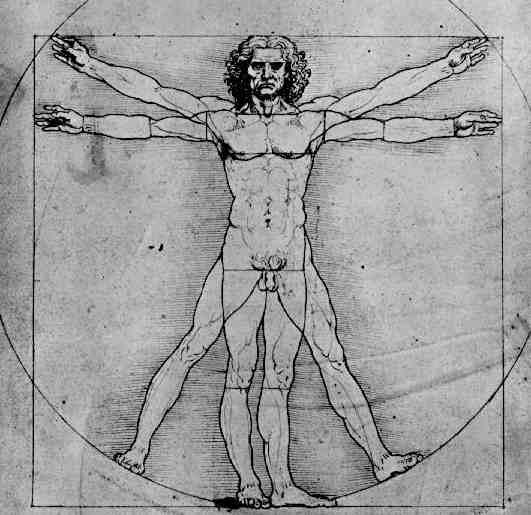
\includegraphics[height=50mm]{Figs/da-vinci-man.jpg}
\end{minipage}
\hspace{15mm}
\begin{minipage}[t]{50mm}
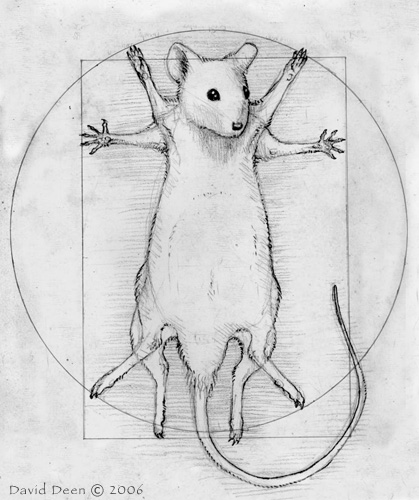
\includegraphics[height=50mm]{Figs/vitruvian_mouse.jpg}
\hspace{5mm}
\href{http://daviddeen.com}{\scriptsize \lolit \tt daviddeen.com}
\end{minipage}
}
\end{frame}


\begin{frame}[c]{Intercross}
\figh{Figs/intercross.pdf}{1.0}
\end{frame}


\begin{frame}[c]{Data}

\hspace{0mm}

\figw{Figs/data_fig.png}{1.15}
\end{frame}



\begin{frame}[c]{QTL mapping}

\vspace{5mm}
\figh{Figs/lodcurve_insulin_with_effects.pdf}{0.75}
\end{frame}


\begin{frame}[c]{Interactive plot}

\vspace{8mm}

\figh{Figs/lod_interactive.png}{0.7}

\vspace{3mm}

\hfill
\href{https://bit.ly/lod_and_effect}{\scriptsize
  \lolit \tt bit.ly/lod\_and\_effect}

\end{frame}


\begin{frame}[c]{17 years of R/qtl}

\figw{Figs/rqtl_lines_code.pdf}{1.0}

\end{frame}



\begin{frame}[c]{}

\centerline{\Large Good things}

\vspace{4mm}

\onslide<2>{
\begin{itemize}
\lolit
  \item some of the code
  \item basics of the user interface
  \item diagnostics and data visualization
  \item quite comprehensive
  \item quite flexible
\end{itemize}
}

\end{frame}


\begin{frame}{}

\vspace*{16.7mm}

\centerline{\Large Bad things}

\end{frame}


\begin{frame}[c]{Input file}

\figh{Figs/datafile.pdf}{0.6}

\end{frame}


\begin{frame}[c,fragile]{Stupidest code ever}

\begin{center}
\begin{minipage}[c]{9.3cm}
\begin{semiverbatim}
\lstset{basicstyle=\normalsize}
\begin{lstlisting}[linewidth=9.3cm]
n <- ncol(data)
temp <- rep(FALSE,n)
for(i in 1:n) {
  temp[i] <- all(data[2,1:i]=="")
  if(!temp[i]) break
}
if(!any(temp)) stop("...")
n.phe <- max((1:n)[temp])
\end{lstlisting}
\end{semiverbatim}
\end{minipage}
\end{center}

\vspace{3mm}

\hfill \href{http://kbroman.org/blog/2011/08/17/the-stupidest-r-code-ever}{\scriptsize \lolit \tt kbroman.org/blog/2011/08/17/the-stupidest-r-code-ever}

\end{frame}


\begin{frame}[c]{}

  \large

  {\hilit Open source} {\lolit means}

  everyone can see my stupid mistakes

  \bigskip \bigskip \bigskip

  \onslide<2>{
    {\hilit Version control} {\lolit means}

  everyone can see every stupid mistake I've ever made
}

\end{frame}


\begin{frame}{}

\vspace*{16.7mm}

\centerline{\Large Documentation}

\end{frame}



\begin{frame}{}

\vspace*{16.7mm}

\centerline{\Large Support}

\end{frame}



\begin{frame}[c]{QTL mapping}

\vspace{5mm}
\figh{Figs/lodcurve_insulin_with_effects.pdf}{0.9}
\end{frame}



\begin{frame}[c]{Congenic line}

\figw{Figs/congenic.pdf}{1.0}

\end{frame}



\begin{frame}[c]{Improving precision}

  \vspace{-20mm}

  \bbi
\item more recombinations
\item more individuals
\item more precise phenotype
\item lower-level phenotypes
\bi
\item transcripts, proteins, metabolites
  \ei
  \ei

\end{frame}



\begin{frame}[c]{Advanced intercross lines}

  \figh{Figs/ail.pdf}{0.9}

\end{frame}


\begin{frame}[c]{Recombinant inbred lines}

  \figh{Figs/rilines.pdf}{0.9}

\end{frame}


\begin{frame}[c]{Collaborative Cross}

  \figh{Figs/ri8.pdf}{0.9}

\end{frame}



\begin{frame}[c]{Heterogeneous stock}

  \vspace{2mm}

  \figh{Figs/hs.pdf}{0.9}

\end{frame}


\begin{frame}[c]{Genome-scale phenotypes}

\figh{Figs/mouse_on_chips.png}{0.75}

\end{frame}



\begin{frame}{Challenges: {\color{foreground} diagnostics}}

\vspace{2mm}

\figw{Figs/weird_correlation_matrix.png}{0.65}

\vspace{3mm}

\hfill \href{http://kbroman.org/blog/2012/04/25/microarrays-suck}{\scriptsize \lolit \tt kbroman.org/blog/2012/04/25/microarrays-suck}

\end{frame}


\begin{frame}{Challenges: {\color{foreground} diagnostics}}

  \vspace{8mm}

\figw{Figs/many_boxplots.png}{0.85}

\vspace{3mm}

\hfill
\href{https://bit.ly/many_boxplots}{\scriptsize
  \lolit \tt bit.ly/many\_boxplots}

\end{frame}


\begin{frame}[c]{Challenges: {\color{foreground} diagnostics}}

\vspace{-20mm}

  \bbi
\item What might have gone wrong?
\item How might it be revealed?
\item Make lots of graphs
\item Follow up artifacts
  \ei

\end{frame}


\begin{frame}[c]{Challenges: {\color{foreground} scale of results}}

\only<1>{\figw{Figs/scale_fig1.pdf}{1.0}}
\only<2>{\figw{Figs/scale_fig2.pdf}{1.0}}

\end{frame}




\begin{frame}[c]{Challenges: {\color{foreground} organizing, automating}}

\only<1>{\figw{Figs/batches_fig1.pdf}{1.0}}
\only<2>{\figw{Figs/batches_fig2.pdf}{1.0}}
\only<3>{\figw{Figs/batches_fig3.pdf}{1.0}}
\only<4>{\figw{Figs/batches_fig4.pdf}{1.0}}
\only<5>{\figw{Figs/batches_fig5.pdf}{1.0}}
\only<6>{\figw{Figs/batches_fig6.pdf}{1.0}}
\only<7>{\figw{Figs/batches_fig7.pdf}{1.0}}

\end{frame}


\begin{frame}[c]{Challenges: {\color{foreground} metadata}}


  \centerline{What the heck is {\hilit \tt "FAD\_NAD SI 8.3\_3.3G"}?}

\end{frame}



\begin{frame}[c]{}
\centerline{\Large What was the question again?}
\end{frame}



\begin{frame}[c]{}

  \vspace*{5mm}

\figh{Figs/rqtl2_3d.png}{0.85}


\vspace{3mm}

\hfill \href{https://ropenscilabs.github.io/miner_book}{\scriptsize \lolit \tt ropenscilabs.github.io/miner\_book}

\end{frame}



\begin{frame}[c]{R/qtl2}

\vspace*{-16.2mm}

  \vspace{21mm}

  \bbi
\item High-density genotypes
\item High-dimensional phenotypes
\item Multi-parent populations
\item Linear mixed models
  \ei

  \vspace{25mm}

\hfill \href{http://kbroman.org/qtl2}{\small \tt kbroman.org/qtl2}

\end{frame}



\begin{frame}[c]{R/qtl2: \color{foreground} Let's not make the same mistakes}

  \bbi
\only<1>{
\item C++ and Rcpp
\item Roxygen2 for documentation
\item Unit tests
\item A single ``switch'' for cross type
}
\only<2>{
{\lolit
\item C++ and Rcpp
\item Roxygen2 for documentation
\item Unit tests
\item A single ``switch'' for cross type
}
}
\onslide<2>{
\item Split into multiple packages
\item Yet another data input format
\item Flatter data structures, but still complex
}
\ei

\end{frame}



\begin{frame}{}

\vspace*{16.7mm}

\centerline{\Large Sustainable academic software}

\end{frame}







\begin{frame}[c]{Acknowledgments}

\begin{columns}[T]
  \begin{column}[T]{0.5\textwidth}
    \vspace{0pt}
\bi
\item[] Danny Arends
\item[] Gary Churchill
\item[] Nick Furlotte
\item[] Dan Gatti
\item[] Ritsert Jansen
\item[] Pjotr Prins
\item[] \'Saunak Sen
\item[] Petr Simecek
\item[] Artem Tarasov
\item[] Hao Wu
\item[] Brian Yandell
  \ei
  \end{column} \hfill
\begin{column}[T]{0.5\textwidth}
\vspace*{0mm}

  \bi
\item[] Robert Corty
\item[] Timoth\'ee Flutre
\item[] Lars Ronnegard
\item[] Rohan Shah
\item[] Laura Shannon
\item[] Quoc Tran
\item[] Aaron Wolen
\item[]
\item[] NIH/NIGMS
  \ei
\end{column}
\end{columns}

\end{frame}


\begin{frame}[c]{}

\Large

Slides: \href{http://bit.ly/uchi2017}{\tt bit.ly/uchi2017} \quad

\includegraphics[height=5mm]{Figs/cc-zero.png}

\vspace{7mm}

\href{http://kbroman.org}{\tt \lolit kbroman.org}

\vspace{7mm}

\href{http://kbroman.org/qtl2}{\tt kbroman.org/qtl2}

\vspace{7mm}

\href{https://github.com/kbroman}{\tt \lolit github.com/kbroman}

\vspace{7mm}

\href{https://twitter.com/kwbroman}{\tt \lolit @kwbroman}


\end{frame}




\end{document}
